\documentclass[journal,12pt,twocolumn]{IEEEtran}

\usepackage{setspace}
\usepackage{amssymb}
\usepackage{amsthm}
\usepackage{mathrsfs}
\usepackage{enumitem}
\usepackage{mathtools}
\usepackage{float}
\usepackage{caption}
\usepackage{graphicx}
\usepackage[breaklinks=true]{hyperref}

\usepackage{listings}
    \usepackage{color}                                            %%
    \usepackage{array}                                            %%
    \usepackage{longtable}                                        %%
    \usepackage{calc}                                             %%
    \usepackage{multirow}                                         %%
    \usepackage{hhline}                                           %%
    \usepackage{ifthen}                                           %%
    \usepackage{lscape}     
    \usepackage{amsmath}
       
\lstset{
%language=C,
frame=single, 
breaklines=true,
columns=fullflexible
}
\def\inputGnumericTable{}
\bibliographystyle{IEEEtran}

\newcommand{\question}{\noindent \textbf{Question: }}
\newcommand{\solution}{\noindent \textbf{Solution: }}
\providecommand{\pr}[1]{\ensuremath{\Pr\left(#1\right)}}
\providecommand{\cbrak}[1]{\ensuremath{\left\{#1\right\}}}
\providecommand{\brak}[1]{\ensuremath{\left(#1\right)}}
\newcommand{\mydet}[1]{\ensuremath{\begin{vmatrix}#1\end{vmatrix}}}
\newcommand{\myvec}[1]{\ensuremath{\begin{pmatrix}#1\end{pmatrix}}}
\newcommand*{\permcomb}[4][0mu]{{{}^{#3}\mkern#1#2_{#4}}}
\newcommand*{\perm}[1][-3mu]{\permcomb[#1]{P}}
\newcommand*{\comb}[1][-1mu]{\permcomb[#1]{C}}

\title{Assignment 5}
\author{AKHILA, CS21BTECH11031}

\begin{document}
% make the title area
\maketitle
\question
The probability of a shooter hitting a target is $\frac{3}{4}$. How many minimum
number of times must he/she fire so that the probability of hitting the target at least
once is more than 0.99?\\

\solution Let the shooter fire $n$ times. Obviously, $n$ fires are $n$ Bernoulli trials.\\
In each trial,\\
p = probability of hitting the target =$\frac{3}{4}$ \\
q = probability of not hitting the target =$\frac{1}{4}$.\\

Let $X$ be the random variable whose probability distribution is B\brak{n,\frac{3}{4}}.\\
We know that,
\begin{align}
\pr{X=k}&=\myvec{n \\ k}q^{n-k}p^k ,k=0,1,2,\dots n\\
    &=\myvec{n \\ k}\brak{\frac{1}{4}}^{n-k}\brak{\frac{3}{4}}^k\\
    &=\myvec{n \\ k}\frac{3^k}{4^n}
\end{align}
Now, given that,
\begin{align}
\pr{\text {hitting the target at least once}} > 0.99\\
\implies \pr{X\geq 1} > 0.99
\end{align}
\begin{multline}
\implies \pr{X=1}+\pr{X=2}+\dots \\ ..+\pr{X=n} > 0.99
\end{multline}
\begin{align}
&\implies 1-\pr{X=0} > 0.99\\
&\implies 1-\myvec{n \\ 0}\frac{3^0}{4^n} > 0.99\\
&\implies 1-\myvec{n \\ 0}\frac{1}{4^n} > 0.99\\
&\implies \myvec{n \\ 0}\frac{1}{4^n} < 0.01\\
&\implies \frac{1}{4^n} < 0.01\\
&\implies 4^n > 100
\end{align}
The minimum value of $n$ to satisfy the above inequality is 4.\\
Thus, the shooter must fire 4 times.
\begin{figure}[H]
    \centering
    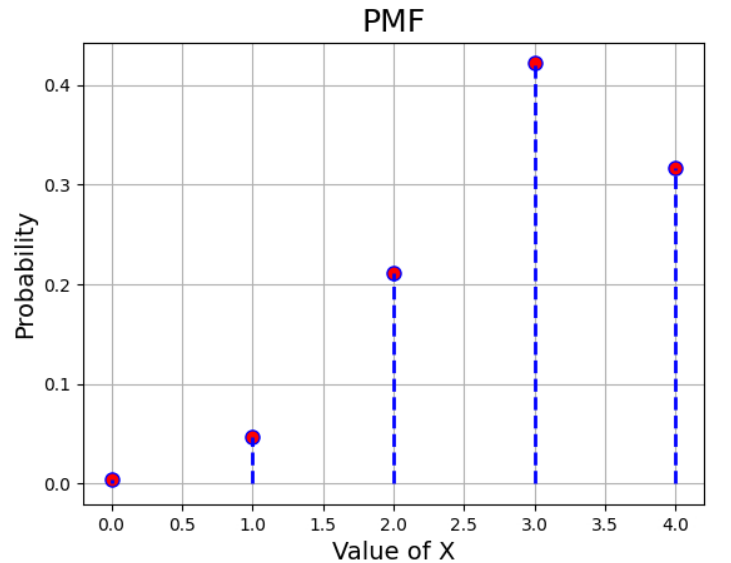
\includegraphics[width=\columnwidth]{plot5.png}
    \captionsetup{justification=centering,margin=1cm}
    \caption{Plot of the PMF}
    \label{fig:plot5}
\end{figure}
\end{document}